% Preamble
% ---
\documentclass{article}

% Packages
% ---
\usepackage{amsmath} % Advanced math typesetting
\usepackage[utf8]{inputenc} % Unicode support (Umlauts etc.)
\usepackage{hyperref} % Add a link to your document
\usepackage{graphicx} % Add pictures to your document
\usepackage{subfig}
\usepackage{listings} % Source code formatting and highlighting
\usepackage{float}
\usepackage[margin=2cm]{geometry}


\title{Guía de uso de Lattice Radiant Software}
\date{2019-Octubre}
\author{Electrónica 3}

\begin{document}

\maketitle
\pagenumbering{gobble}
\newpage
\pagenumbering{arabic}

\tableofcontents
\pagebreak

%Empiezan las secciones del articulo

\section{Descarga e instalación}
El software utilizado para programar la FPGA provista por la cátedra es 'Lattice Radiant Software'.El mismo puede descargarse tanto para Linux como para Windows del siguiente link: \url{https://tinyurl.com/y46mth4j}
\subsection{ Elección del sistema operativo}

\begin{figure}[H]
\centering
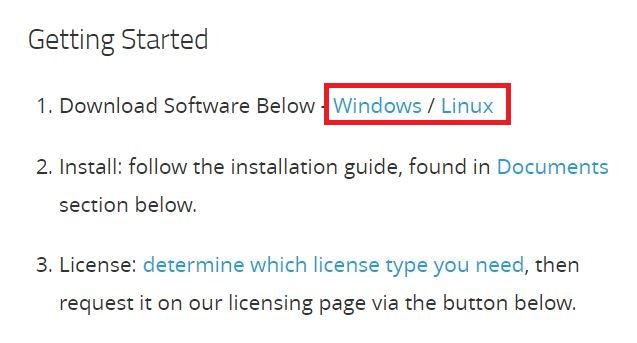
\includegraphics[width=0.4\linewidth]{Imagenes/1.JPG}
\caption{Guía de descarga: Paso 1}
\label{fig:step1}
\end{figure}


\subsection{ Ejemplo de selección: caso Windows}

\begin{figure}[H]
\centering
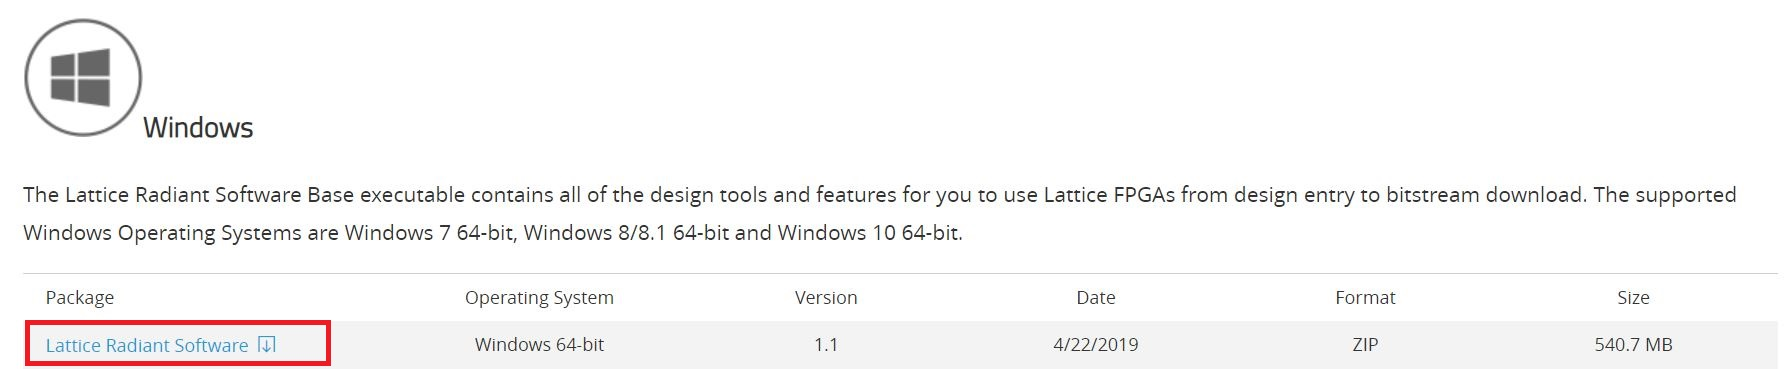
\includegraphics[width=1\linewidth]{Imagenes/2.JPG}
\caption{Guía de descarga: Paso 2}
\label{fig:step2}
\end{figure}

\subsection{Sign in request}
Después de haber seleccionado Lattice Radiant Software, nos lleva una página donde para poder entrar tenemos que estar registrados.

\begin{figure}[H]
\centering
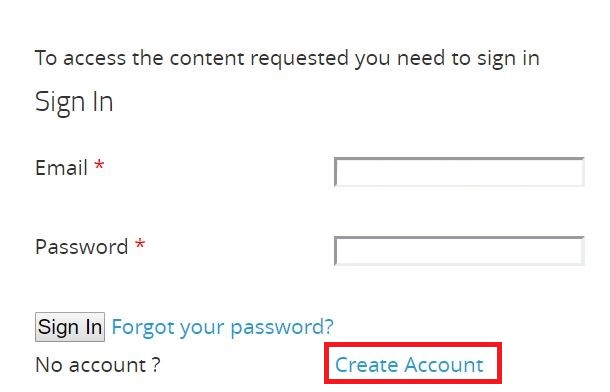
\includegraphics[width=0.4\linewidth]{Imagenes/3.JPG}
\caption{Guía de descarga: Paso 3}
\label{fig:step3}
\end{figure}

Para poder seguir, procedemos a registrarnos

\subsection{Registration}
A continuación dejamos una captura de cómo hay que rellenar ciertos campos específicos. Sugerimos utilizar el mail del itba a la hora de registrarse.

\begin{figure}[H]
\centering
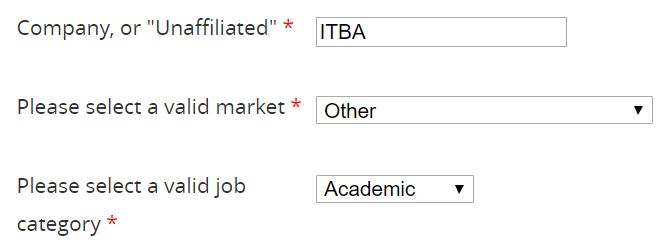
\includegraphics[width=0.4\linewidth]{Imagenes/4.JPG}
\caption{Guía de descarga: Paso 4}
\label{fig:step4}
\end{figure}

\subsection{Descarga}
Ahora que tenemos una cuenta, volvemos a la página de lattice para proceder con la descarga. En esa página, aceptamos términos y condiciones, y a continuación clickeamos en Download.

\begin{figure}[H]
\centering
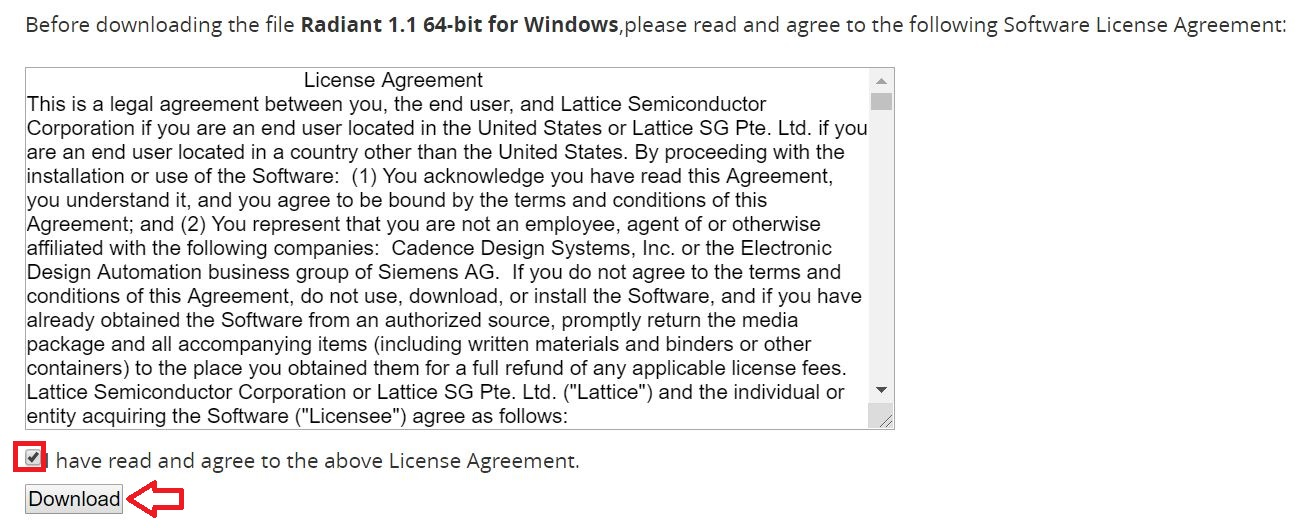
\includegraphics[width=1\linewidth]{Imagenes/5.JPG}
\caption{Guía de descarga: Paso 5}
\label{fig:step5}
\end{figure}

\subsection{Instalación}
\subsubsection{Ejecutar el archivo .exe}

Descomprimimos el archivo descargado y ejecutamos el archivo .exe que se encuentra dentro de la carpeta
\begin{figure}[H]
\centering
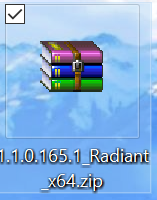
\includegraphics[width=0.1\linewidth]{Imagenes/zip.PNG}
\caption{Archivo a descomprimir}
\label{fig:install}
\end{figure}

\newpage

\subsubsection{Capturas de instalación}

\begin{figure}[H]
\centering
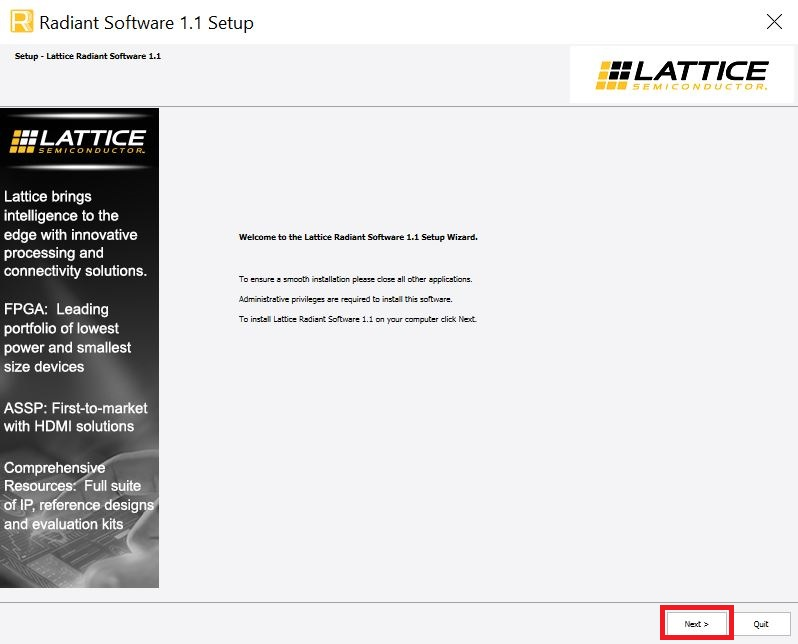
\includegraphics[width=0.8\linewidth]{Imagenes/inst1.JPG}
\caption{Instalación: captura 1 }
\label{fig:install}
\end{figure}

\begin{figure}[H]
\centering
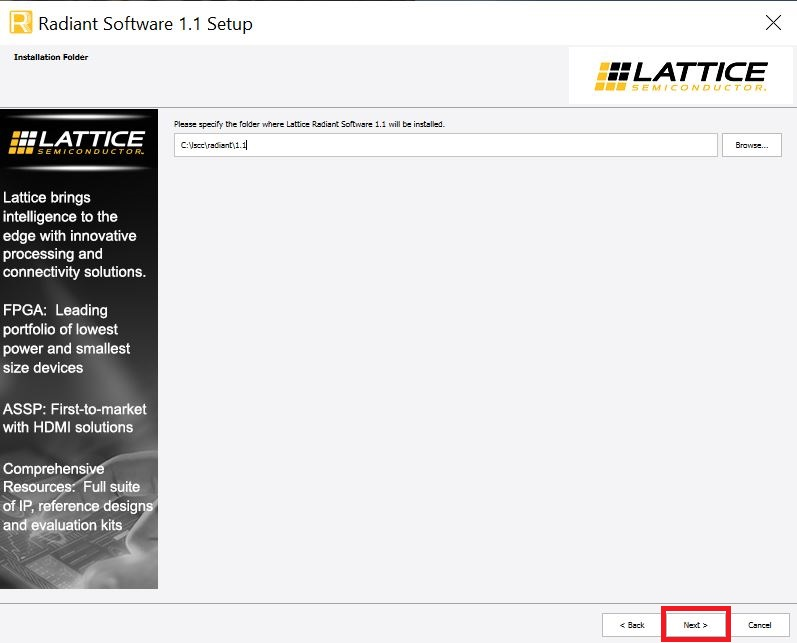
\includegraphics[width=0.8\linewidth]{Imagenes/inst2.JPG}
\caption{Instalación: captura 2 }
\label{fig:install}
\end{figure}

\begin{figure}[H]
\centering
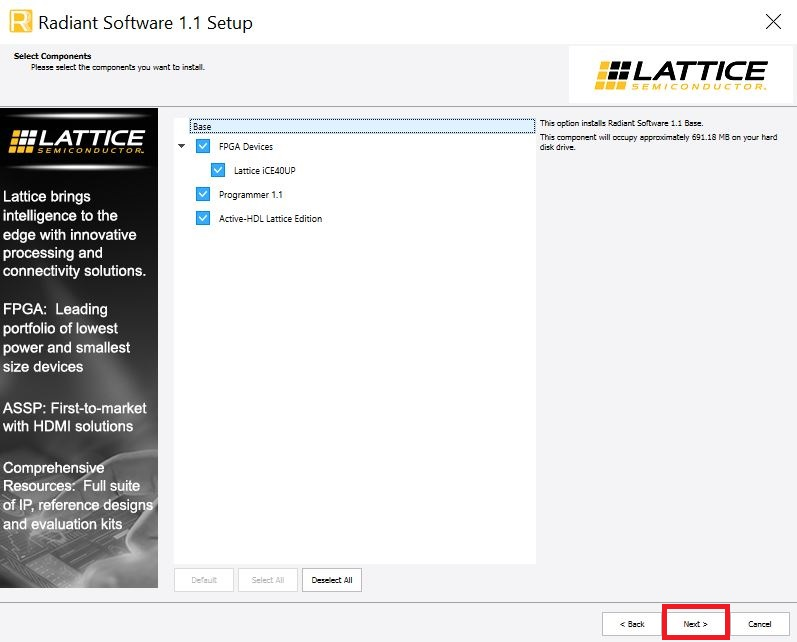
\includegraphics[width=0.8\linewidth]{Imagenes/inst3.JPG}
\caption{Instalación: captura 3 }
\label{fig:install}
\end{figure}

\begin{figure}[H]
\centering
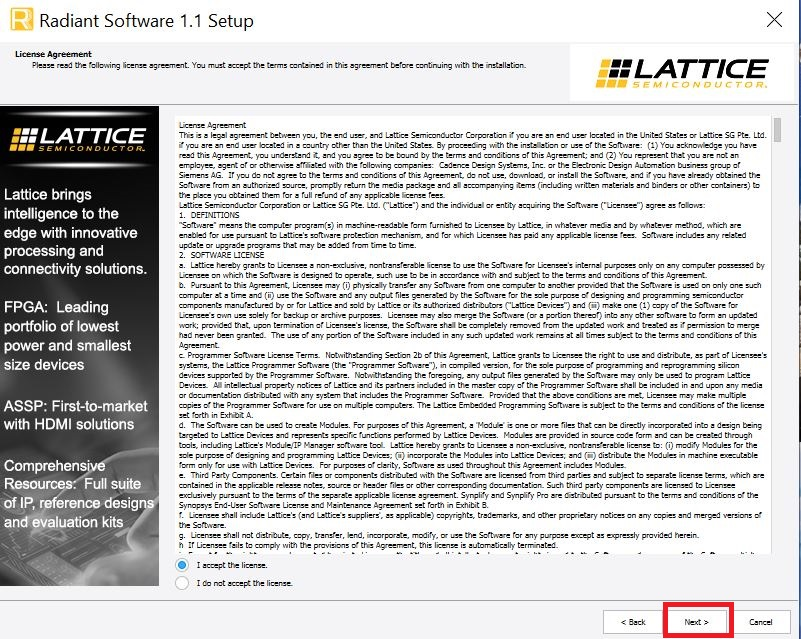
\includegraphics[width=0.8\linewidth]{Imagenes/inst4.JPG}
\caption{Instalación: captura 4 }
\label{fig:install}
\end{figure}

\begin{figure}[H]
\centering
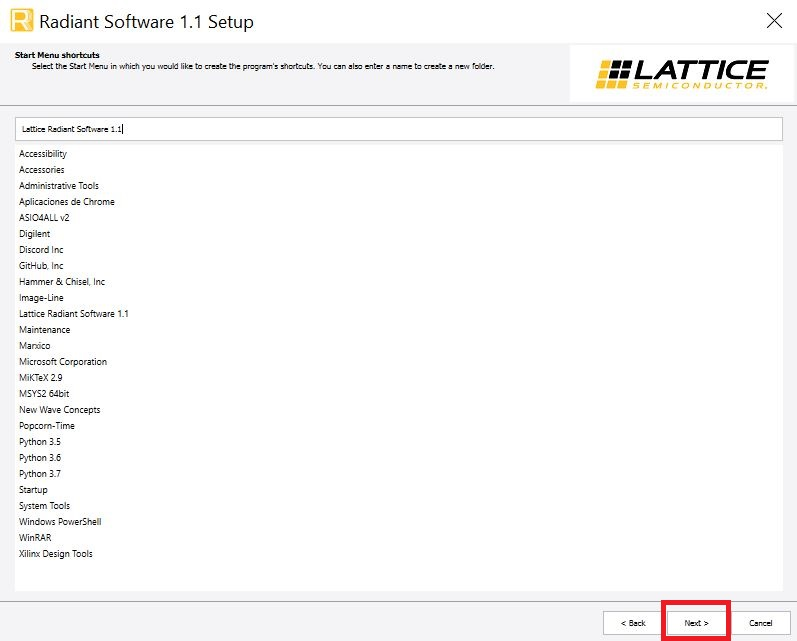
\includegraphics[width=0.8\linewidth]{Imagenes/inst5.JPG}
\caption{Instalación: captura 5 }
\label{fig:install}
\end{figure}

\begin{figure}[H]
\centering
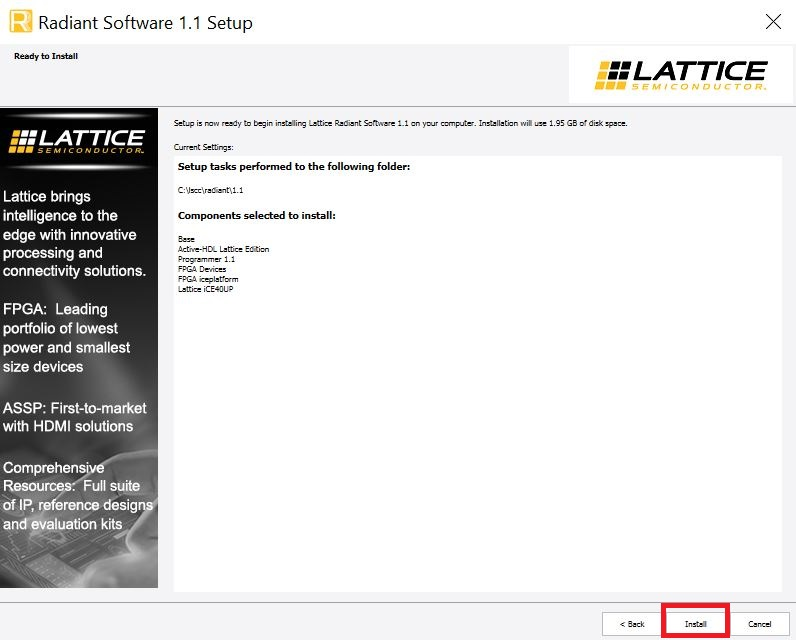
\includegraphics[width=0.8\linewidth]{Imagenes/inst6.JPG}
\caption{Instalación: captura 6 }
\label{fig:install}
\end{figure}


\begin{figure}[H]
\centering
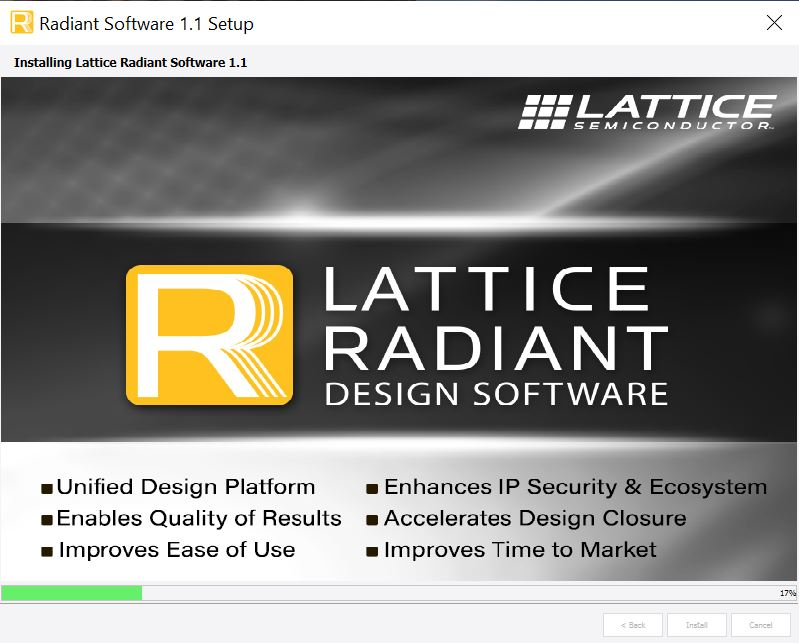
\includegraphics[width=0.8\linewidth]{Imagenes/inst7.JPG}
\caption{Instalación: captura 7 }
\label{fig:install}
\end{figure}


\begin{figure}[H]
\centering
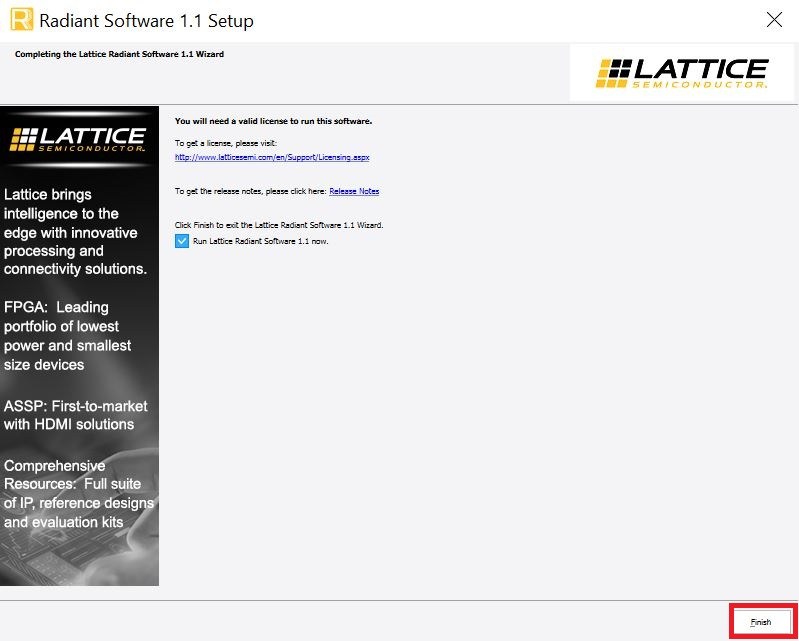
\includegraphics[width=0.8\linewidth]{Imagenes/inst8.JPG}
\caption{Instalación: captura 8 }
\label{fig:install}
\end{figure}



\subsection{Licencia}
Para tener una licencia, hay que generar una solicitud en
\href{https://www.latticesemi.com/Support/Licensing}{https://www.latticesemi.com/Support/Licensing}.
En esa página, vamos la parte de Lattice Radiant Software y clickeamos en Request a Free License.

\begin{figure}[H]
\centering
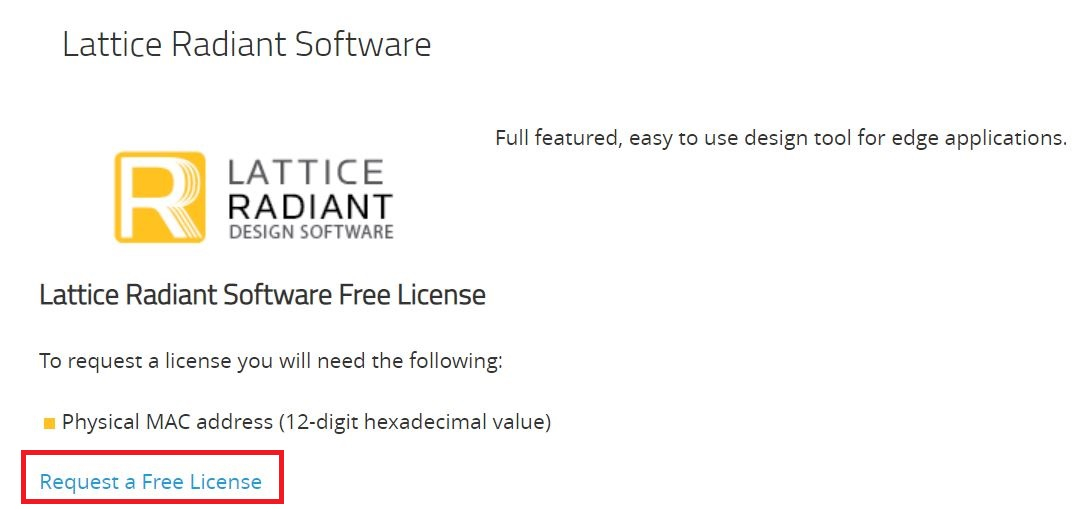
\includegraphics[width=1\linewidth]{Imagenes/6.JPG}
\caption{Guía de descarga: Paso 6}
\label{fig:step6}
\end{figure}

El proceso puede demorar 1 día así que hay que procurar no hacerlo a último momento.

\section{Creación de un proyecto}
	Para crear un nuevo proyecto se debe abrir el programa recientemente instalado y elegir 'New Project'.
	\begin{figure}[H]
	\centering
	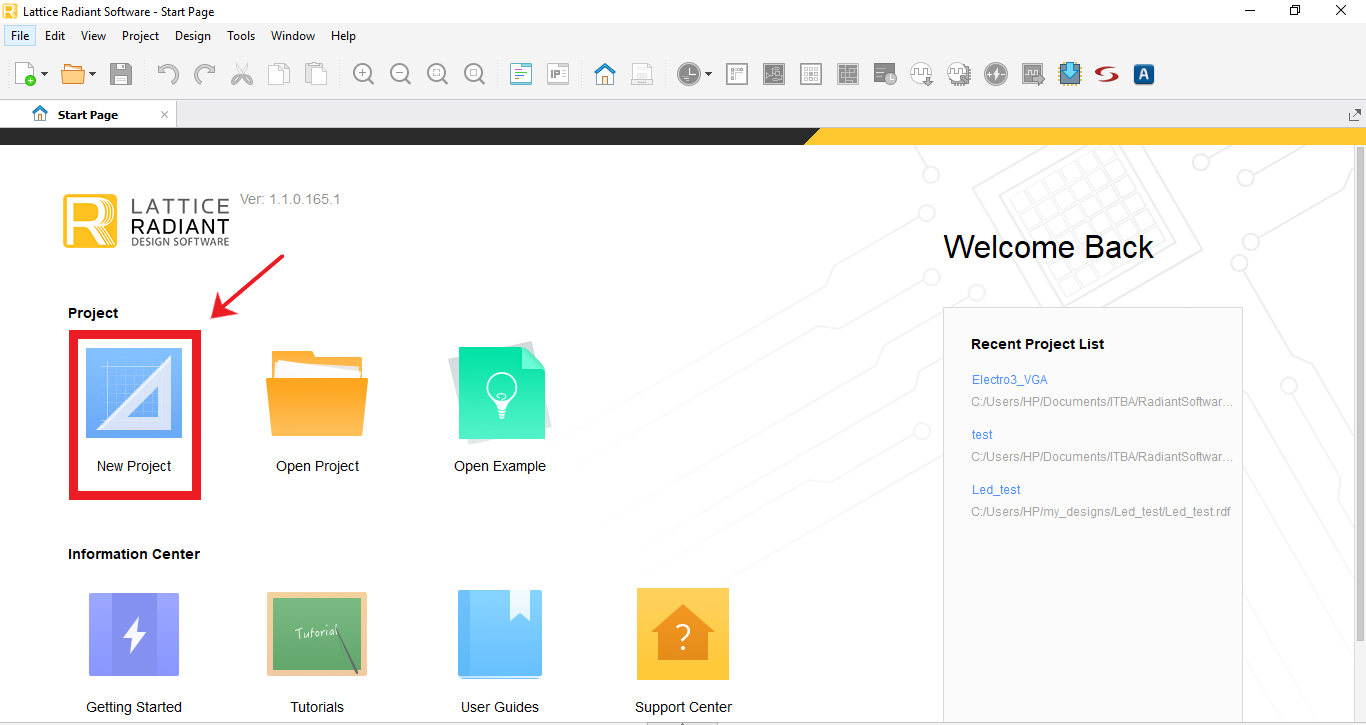
\includegraphics[height=6cm,width=0.7\linewidth]{Imagenes/NewProj.png}
	\caption{Opción para crear un nuevo proyecto}
	\end{figure}
	
	Luego de hacer click en New Project y en el botón de next, se debe elegir el nombre del proyecto y en que carpeta se desea guardar.Dejar el nombre bajo el campo de "Implementation" en su valor default y hacer click en next nuevamente.
	En la siguiente ventana se puede elegir agregar archivos al nuevo proyecto.En este paso se puede elegir agregar cualquier archivo de Verilog ya existente que sea necesario para el proyecto.
	\begin{figure}[H]
	\centering
	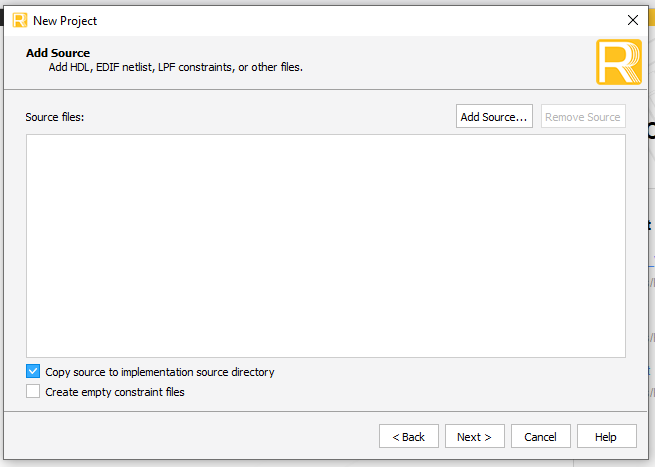
\includegraphics[height=6cm,width=8cm]{Imagenes/AddSources.png}
	\caption{Ventana para agregar archivos ya existentes}
	\end{figure}
	
	Tildar las opciones como se indica en la figura anterior y hacer click en Next.
	En la siguiente ventana se indica el dispositivo a utilizar, completar las opciones igual que como se muestra en la siguiente figura:
	\begin{figure}[H]
	\centering
	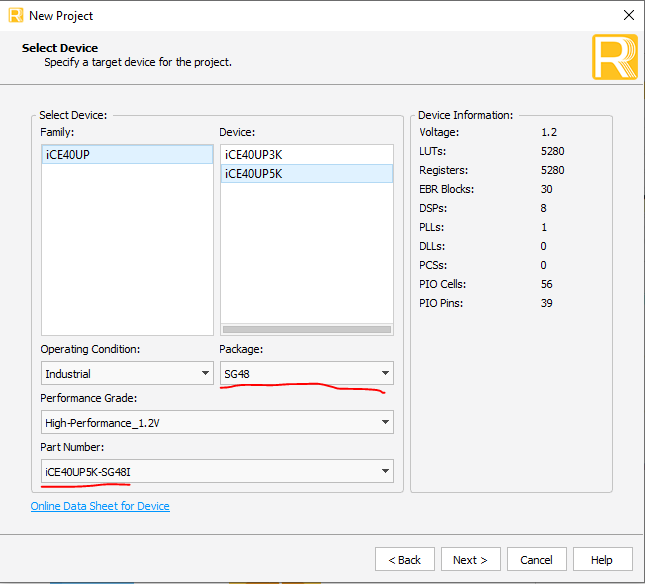
\includegraphics[height=10cm,width=0.8\linewidth]{Imagenes/Dispositivo.png}
	\caption{Prestar especial antencion a que el campo de 'Package' y 'Part Number' coincidan con el de la imagen }
	\end{figure}
	Clickear Next nuevamente, elegir la opción 'Lattice LSE' en la siguiente ventana, elegir next una vez mas y luego Finish.
	

\subsection{Módulos de Verilog}
Se pueden crear/agregar archivos de Verilog al proyecto seleccionando 'File' arriba a la izquierda y luego 'New' para crear un archivo o 'Add' para agregar uno ya existente.

Los archivos de Verilog del proyecto se pueden ver dentro de la carpeta llamada 'Input files'
	\begin{figure}[H]
	\centering
	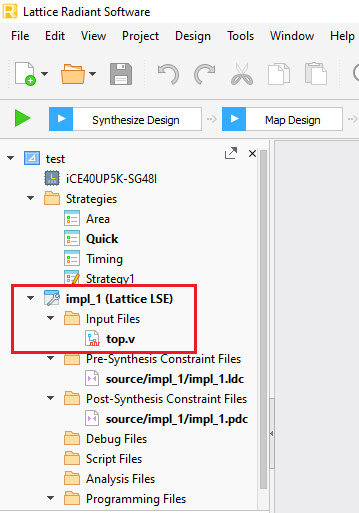
\includegraphics[height=8cm,width=6cm]{Imagenes/VerilogArch.png}
	\caption{Ubicación de los proyectos de Verilog}
	\end{figure}

\subsection{Clocks y timing constraints}
La FPGA utilizada tiene asociado un clock de 12MHz al pin 35 de la misma.Si se desea instanciar un clock de una frecuencia distinta se puede utilizar un modulo de Verilog que funcione para generar clocks mas lentos a partir del de 12MHz o también es posible utilizar primitivas del Radiant.
La FPGA utilizada tiene un oscilador interno de 48MHz el cual puede ser utilizado como clock de 6MHZ, 12MHz, 24MHz o 48MHz mediante la primitiva llamada 'HSOSC'.
	\begin{figure}[H]
	\centering
	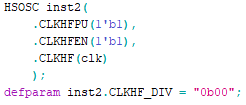
\includegraphics[width=0.3\linewidth]{Imagenes/PrimitivaClk.png}
	\caption{Código de ejemplo de como utilizar la primitiva que utiliza el oscilador interno de 48MHz}
	\end{figure}
	El código anterior debe escribirse en el modulo en el que se define el wire 'clk' que se pasa como  parámetro al puerto CLKHF.El parámetro CLKHFDIV que se define luego de instanciar la primitiva, es el que define la frecuencia del clock a utilizar.Las cuatro opciones para dicho parámetro son:
	\begin{itemize}
	\item CLKHFDIV = "0b00" (Clock de 48MHz)
	\item CLKHFDIV = "0b01" (Clock de 24MHz)
	\item CLKHFDIV = "0b10" (Clock de 12MHz)
	\item CLKHFDIV = "0b11" (Clock de 6MHz)
	\end{itemize}
Es necesario informarle al sintetizador la frecuencia del clock a utilizar, para ello se debe utilizar el 'Timing Constraint Editor'.
	\begin{figure}[H]
	\centering
	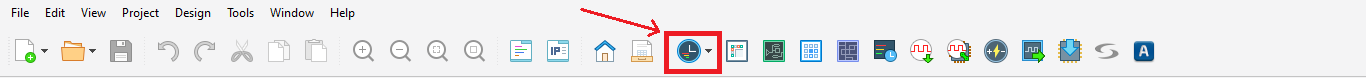
\includegraphics[height=1cm,width=\linewidth]{Imagenes/UbicacionTiming.png}
	\caption{Ubicación del 'Timing constraint editor'}
	\end{figure}
Una vez en la ventana del editor se debe seleccionar la señal utilizada como clock y elegir la frecuencia deseada para el mismo.
	\begin{figure}[H]
	\centering
	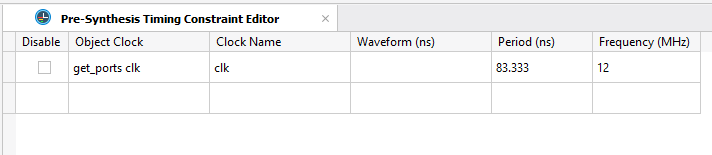
\includegraphics[width=0.7\linewidth]{Imagenes/Clk_ejemplo.png}
	\caption{Ejemplo en el que se utiliza un clock de 12MHz en la señal 'clk'}
	\end{figure}
Es recomendable utilizar directamente el clock de 12MHz asignado al pin 35 de la FPGA.

\section{Simulación}
Para realizar la simulacion del proyecto se debe verificar que todos los archivos de Verilog esten incluidos para la simulacion.
	\begin{figure}[H]
	\centering
	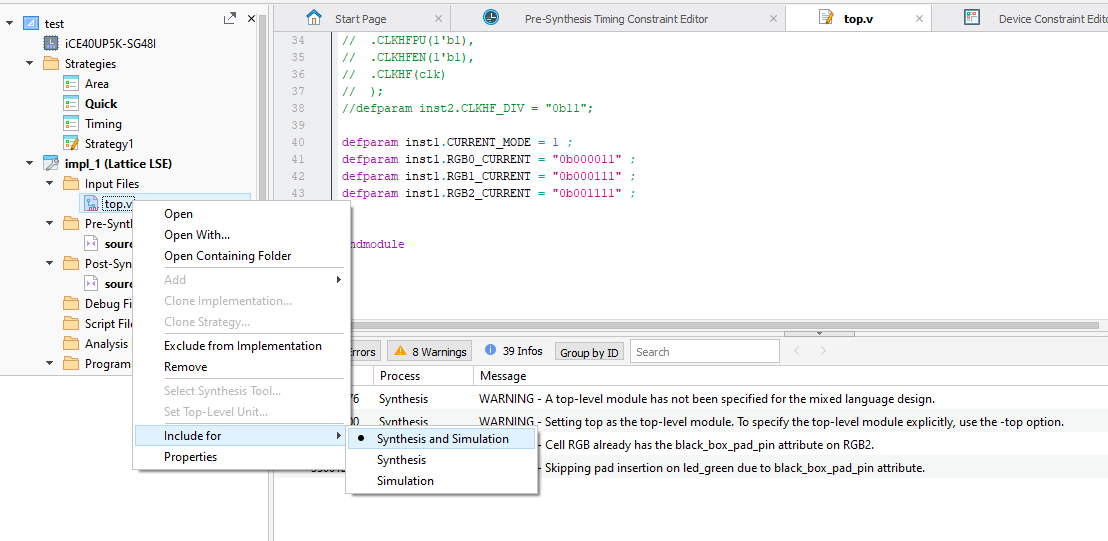
\includegraphics[width=0.8\linewidth]{Imagenes/IncSim.png}
	\caption{Como incluir un archivo a la simulacion}
	\end{figure}
Luego se debe abrir el 'Simulation Wizard' en la parte superior del Radiant
	\begin{figure}[H]
	\centering
	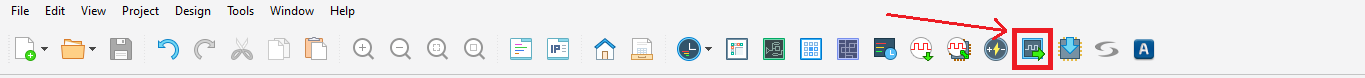
\includegraphics[width=\linewidth]{Imagenes/SimWizardUb.png}
	\caption{Ubicacion del simulation wizard}
	\end{figure}
 y crear un proyecto de simulacion.
 	\begin{figure}[H]
	\centering
	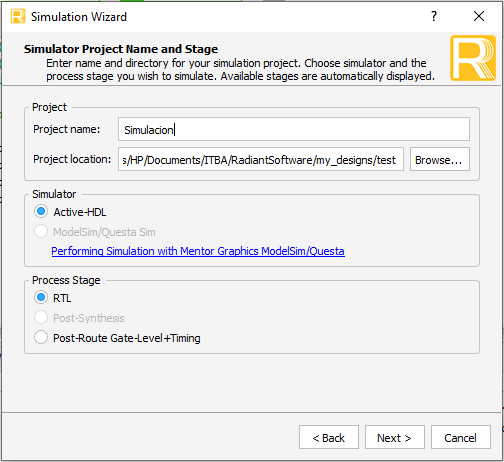
\includegraphics[width=0.5\linewidth]{Imagenes/SimWizard1.png}
	\caption{Elegir en donde guardar los archivos de simulacion y elegir las opciones como se muestra en la imagen}
	\end{figure}
Seleccionar Next hasta llegar a la siguiente ventana y asegurarse que todas las opciones esten elegidas:
	\begin{figure}[H]
	\centering
	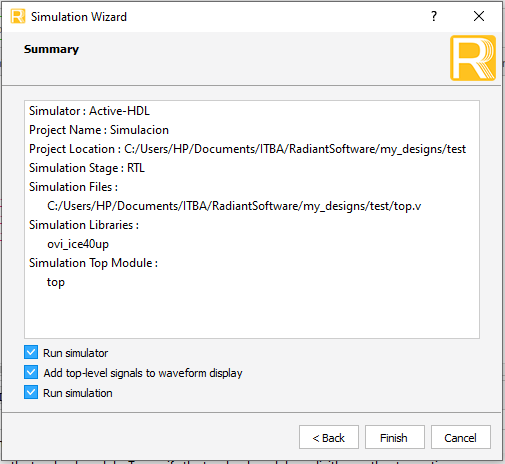
\includegraphics[width=0.5\linewidth]{Imagenes/SimWizard2.png}
	\end{figure}


\section{Asignación de pins}
Para asignar que pin de la FPGA corresponde a que entrada y salida del modulo de Verilog, se debe ir al 'Device Constraint Editor'.
	\begin{figure}[H]
	\centering
	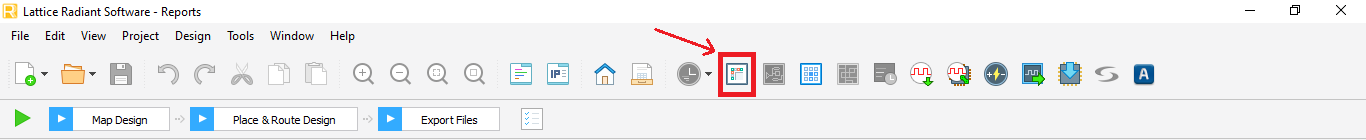
\includegraphics[width=\textwidth]{Imagenes/pins.png}
	\caption{Ubicación del Device Constraint Editor en el Radiant}
	\end{figure}
	
 Una vez abierto el Device Constraint Editor se vera algo similar a lo observado en la siguiente figura:
 	\begin{figure}[H]
 	\centering
	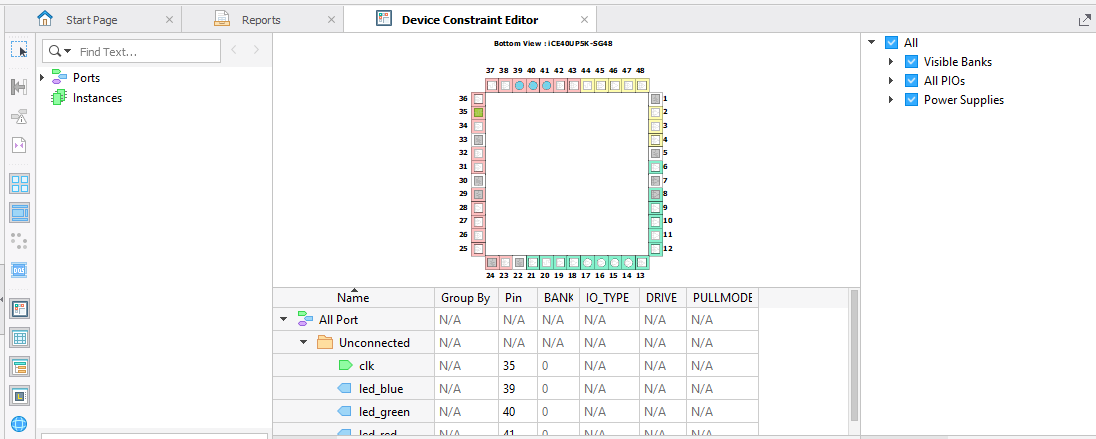
\includegraphics[height=9cm,width=\textwidth]{Imagenes/DeviceConstraintEditor.png}
	\caption{Vista de las señales de Verilog y sus pins correspondientes}
	\end{figure}
 En esta ventana se puede cambiar que pin corresponde a una señal del modulo de Verilog mas alto en la jerarquía.Para realizar cambios solo hace falta hacer click en el campo de 'pin' correspondiente a una señal dada y cambiar el valor numérico.Antes del nombre de cada señal hay una flecha con una dirección y color determinado que indica si la señal es de input o de output.
 
 Hay que tener especial cuidado de asignar pins validos para las señales (utilizar los pins I/O).A continuación se presentan algunas tablas con la función de algunos pins de la FPGA que utiliza la cátedra(ICE40-UP5K).
 \begin{figure}[H]
 \centering
 \subfloat{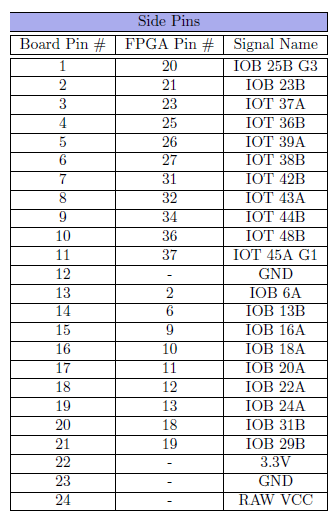
\includegraphics[height=12cm,width=0.5\textwidth]{Imagenes/SidePins.png}\label{fig:f1}}
 \subfloat{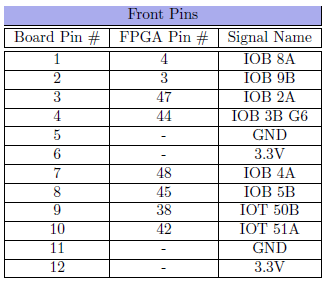
\includegraphics[height=10cm, width=0.5\textwidth]{Imagenes/FrontPins.png}\label{fig:f2}}
	\end{figure}
	

\section{Compilación,síntesis y programador}
Para cargar el programa en Verilog a la FPGA se deben seguir los pasos de síntesis, mappeo, routeo y exportación que aparecen arriba de la ventana de archivos.
	\begin{figure}[H]
 	\centering
	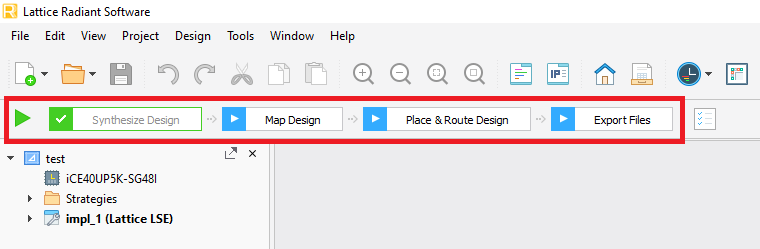
\includegraphics[height=6cm, width=0.8\textwidth]{Imagenes/SintesisRouteo.png}
	\end{figure}
Se puede realizar cada uno de dichos pasos uno por vez o se puede elegir realizar todos clickeando el símbolo verde de play a la izquierda. Ya en el proceso de síntesis el compilador detectara posibles errores de sintaxis en el código de Verilog así como también los warnings.

Si se desea ver en detalle los resultados de cada paso se puede ir a 'view' en la parte de arriba y luego seleccionar reports.
	\begin{figure}[H]
 	\centering
	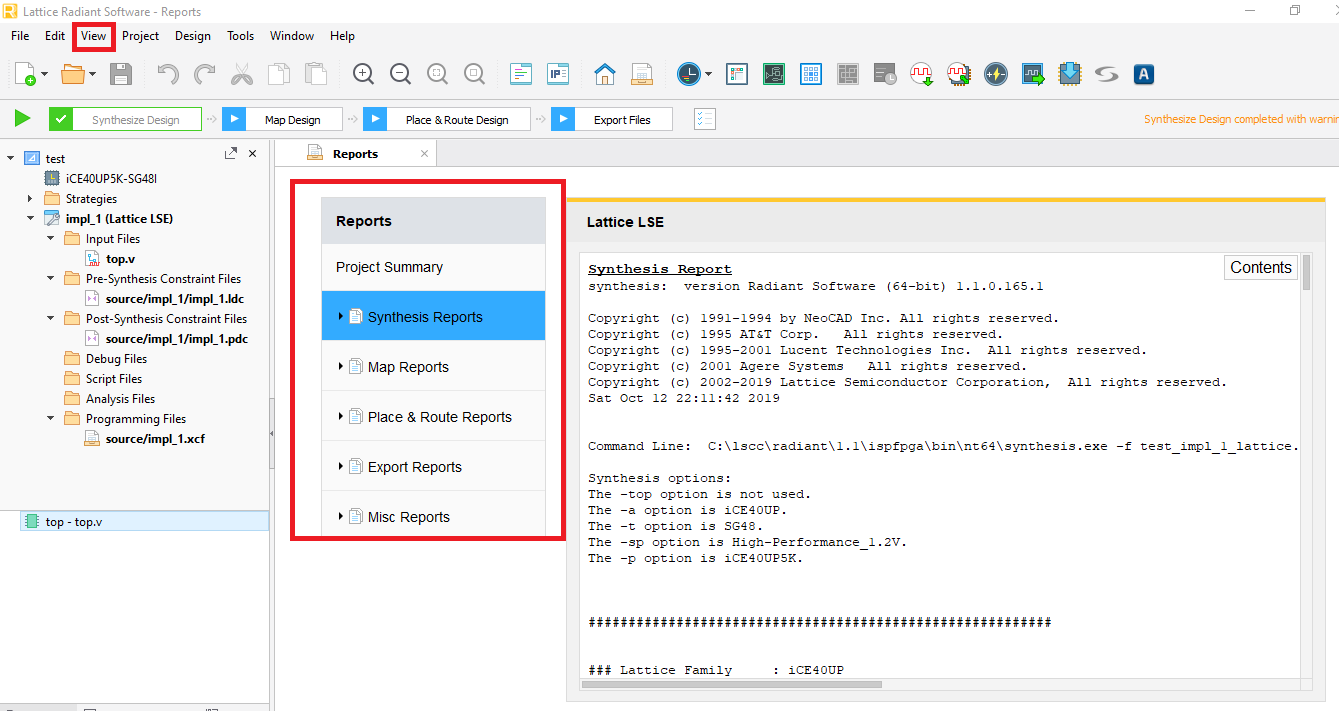
\includegraphics[height=8cm, width=\textwidth]{Imagenes/reports.png}
	\caption{Ventana con los reportes con cada uno de los pasos efectuados}
	\end{figure}
	
Una vez que se consiguieron exitosamente los archivos de salida solo queda cargar los mismos a la FPGA.Para este paso se requiere primero conectar la FPGA a la computadora mediante un cable USB a Micro USB.Luego de conectar la FPGA se debe abrir el programmer el cual esta ubicado en la parte superior derecha del lattice como se indica en la siguiente figura.
	\begin{figure}[H]
 	\centering
	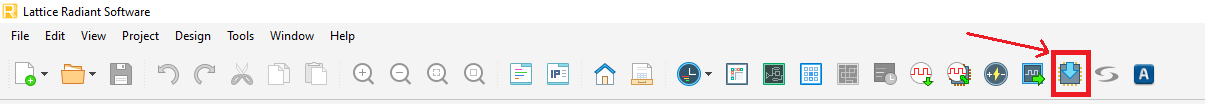
\includegraphics[height=2cm, width=\textwidth]{Imagenes/ProgrammerUbi.png}
	\caption{Ubicación del programmer}
	\end{figure}

Al abrir el programmer con la FPGA ya conectada debería verse algo similar a la siguiente figura:
	\begin{figure}[H]
 	\centering
	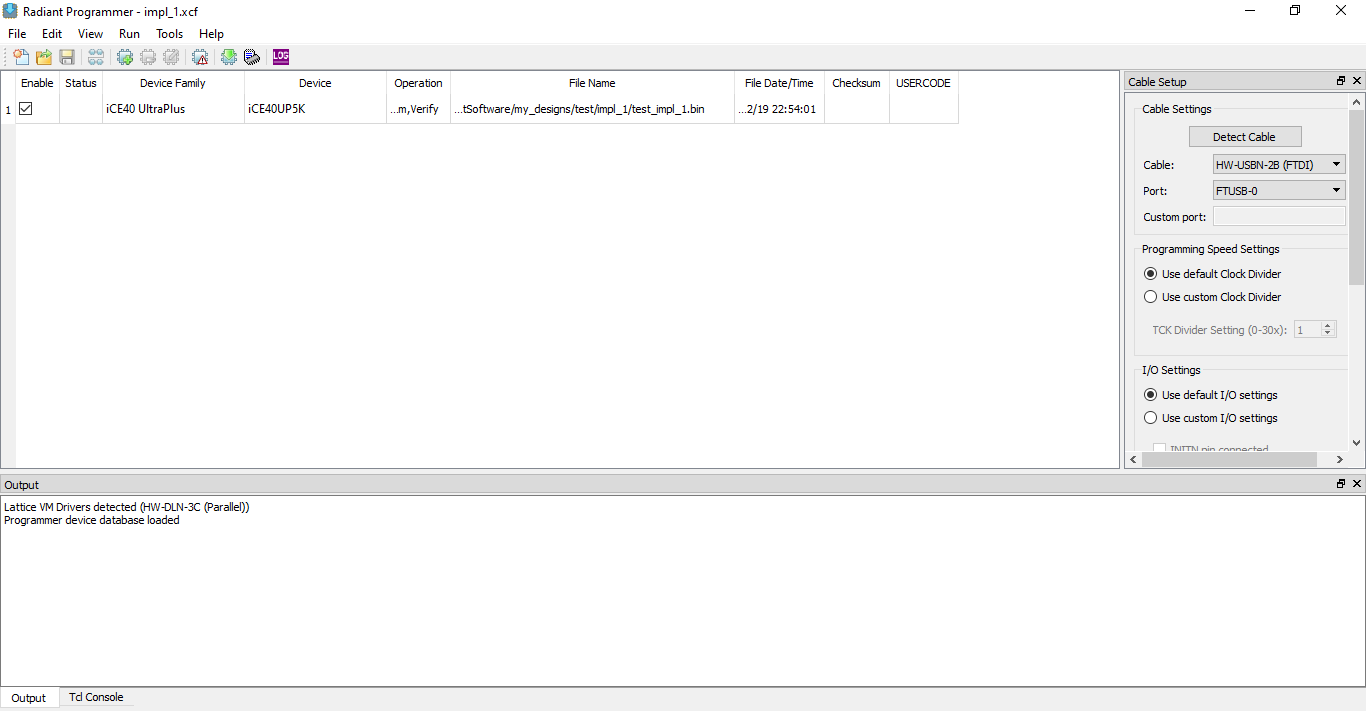
\includegraphics[height=8cm, width=0.8\textwidth]{Imagenes/Programmer.png}
	\caption{Ventana luego de abrir el programmer}
	\end{figure}
Como se puede ver en la figura anterior debería aparecer listada la FPGA que se conecto a la PC. Se puede seleccionar la opción 'Detect Cable' a la derecha para verificar que la computadora reconoció exitosamente la FPGA. Si se tiene problemas con este paso se puede intentar esperar un poco y luego volver a intentar con 'Detect Cable', si esto no funciona se puede probar conectando la FPGA a otro puerto USB de la PC.Por si acaso siempre es mejor conectar y desconectar la FPGA con el programador cerrado y luego volver a abrirlo.

Ahora solo quedo configurar la FPGA.Para eso se debe seleccionar el dispositivo, luego edit y de ahí Device Properties.
	\begin{figure}[H]
 	\centering
	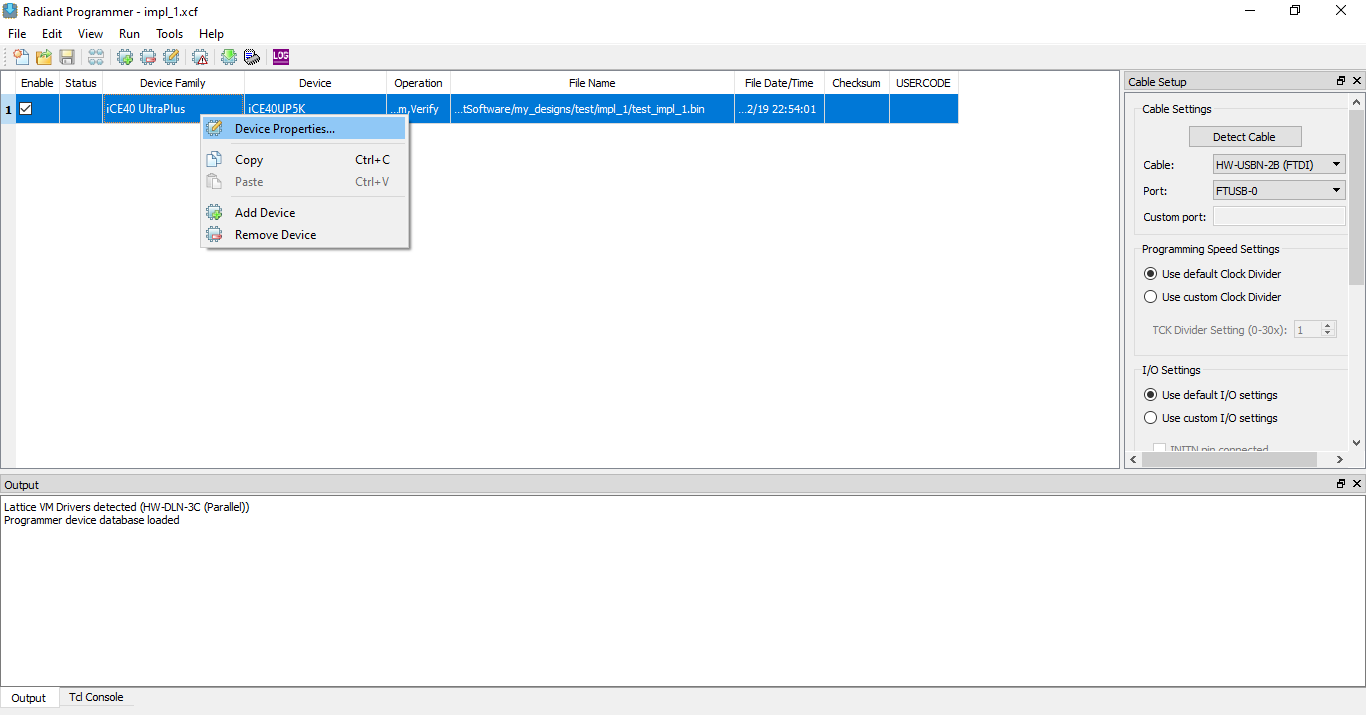
\includegraphics[height=8cm, width=0.9\textwidth]{Imagenes/EditProg.png}
	\end{figure}
Configurar la ventana igual que como se muestra en la siguiente figura:
	\begin{figure}[H]
 	\centering
	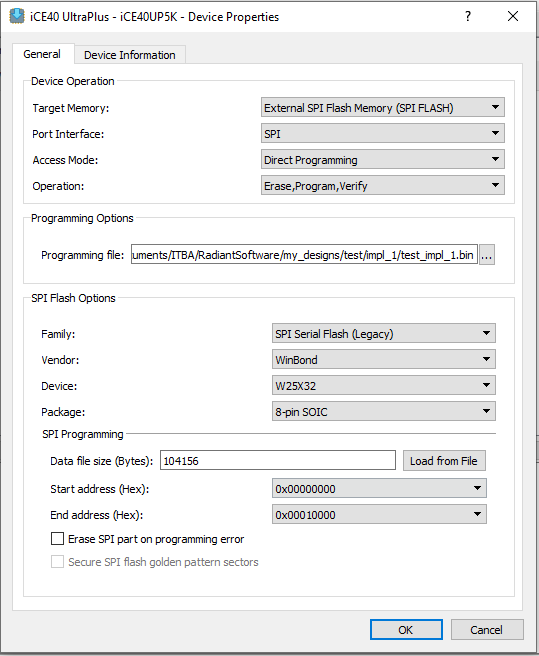
\includegraphics[height=10cm, width=10cm]{Imagenes/Config.png}
	\end{figure}
Para el programming file elegir el archivo con la extension '.bin' resultante de la exportación que se realizo antes de abrir el programmer.Finalmente solo queda subir el .bin a la FPGA seleccionando la opción 'Program Device' que aparece en la barra de arriba.
	\begin{figure}[H]
 	\centering
	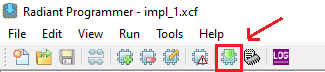
\includegraphics[width=0.8\textwidth]{Imagenes/runprog.png}
	\end{figure}


\end{document}